\chapter{\IfLanguageName{dutch}{Nuxt.js}{Nuxt.js}}
\label{ch:nuxt}
Nuxt.js is een framework voor vue.js applicaties met als doel om vue developers eerste klasse technologieën te laten implementeren zoals server side rendering (SSR), code splitting en pre rendering (\cite{NUXTJS}). Nuxt heeft ook een ingewerkte PWA library. Deze kan gebruikt worden om een site in een PWA te veranderen. 

\section{\IfLanguageName{dutch}{Basisprincipes}{Basisprincipes}}
\label{sec:basisprincipes}

% Server side rendering
\subsection{Server side rendering}
Server side rendering (\cite{NUXT_SERVERSIDERENDERING}) wordt gebruikt om je applicatie te renderen naar statische html en css bestanden. Na het doorsturen van de belangrijkste html en css bestanden worden deze weergegeven op het apparaat. Vervolgens zal de javascript bundel doorgestuurd worden. Dit betekend dat het apparaat geen gebruik kan maken van de javascript functionaliteit zolang deze bundel nog niet gedownload is. Pas na de parsing en uitvoering van de javascript bestand(en) op het apparaat kan hiervan gebruik gemaakt worden.

%Pre rendering
\subsection{Pre rendering}
Pre rendering (\cite{NUXT_PRERENDERING}) is gelijkaardig aan server side rendering. Het grootste verschil is dat pre rendering de pagina zal renderen en deze al opslaan als statisch bestand. Als deze dan wordt opgevraagd door het apparaat zal dit bestand niet nog eens gerenderd worden maar zal de een statische pagina teruggestuurd worden.

%Configuration
\subsection{Configuration}
Het configuration of configuratie (\cite{NUXT_CONFIGURATION}) bestand (nuxt.config.js) is waar alle instellingen van Nuxt geconfigureerd worden.

\begin{lstlisting}[caption=Configuration, language=Javascript]
export default {
	mode: 'universal',
/*
** Headers of the page
*/
	head: {
	title: process.env.npm_package_name || '',
	meta: [
		{ charset: 'utf-8' },
		{ name: 'viewport', content: 'width=device-width, initial-scale=1' },
		{ hid: 'description', name: 'description', content: process.env.npm_package_description || '' }
	],
	link: [
		{ rel: 'icon', type: 'image/png', href: '/icon.png' }
	]
	},
/*
** Customize the progress-bar color
*/
	loading: { color: '#fff' },
/*
** Global CSS
*/
	css: [],
/*
** Plugins to load before mounting the App
*/
	plugins: [],
/*
** Nuxt.js dev-modules
*/
	buildModules: [],
/*
** Nuxt.js modules
*/
	modules: [],
/*
** Build configuration
*/
	build: {
/*
** You can extend webpack config here
*/
		extend (config, ctx) {
		}
	}
}
\end{lstlisting}


%Directory Structure
\subsection{Directory Structure}
Standaard heeft Nuxt.js al een mappen structuur (\cite{NUXT_DIRECTORYSTRUCTURE}). Deze mappenstructuur is een goed beginpunt voor verschillende applicaties om een overzicht binnenin het project te bewaren. Indien de gebruiker deze structuur niet wilt gebruiken is deze vrij om de mappenstructuur aan te passen.

\begin{figure}[!h]
	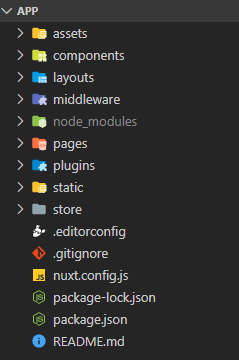
\includegraphics[width=200px]{Nuxt/Nuxt_DirectoryStructure}\centering
	\caption{Voorbeeld mappen structuur nuxt}
\end{figure}


%Routing
\subsection{Routing}
Nuxt.js maakt het heel gemakkelijk om de verschillende routes (\cite{NUXT_ROUTING}) in de site te configureren. Het enige dat de gebruiker hoeft te doen is een map genereren met de naam van de route en een index.vue bestand aanmaken waar nuxt standaard naartoe zal navigeren indien er geen parameters aan te pas komen.

\begin{lstlisting}[caption=Routering mappenstuctuur]
pages/
--| user/
-----| index.vue
-----| one.vue
--| index.vue
\end{lstlisting}

Bovenstaande mappenstructuur zal deze routes genereren:

\begin{lstlisting}[caption=Routering generatie]
router: {
	routes: [
		{
			name: 'index',
			path: '/',
			component: 'pages/index.vue'
		},
		
		{
			name: 'user',
			path: '/user',
			component: 'pages/user/index.vue'
		},
		
		{
			name: 'user-one',
			path: '/user/one',
			component: 'pages/user/one.vue'
		}
	]
}
\end{lstlisting}

Indien er parameters aan te pas komen moet de gebruiker in plaats van een index.vue te creëren een bestand maken met als naam ‘\_ naam van de parameter’. Hierdoor wordt naar deze pagina genavigeerd indien die parameter aanwezig is.

\begin{lstlisting}[caption=Routering mappenstructuur met id parameter]
pages/
--| users/
-----| _id.vue
--| index.vue
\end{lstlisting}

Bovenstaande mappenstructuur zal onderstaande routes genereren: 

\begin{lstlisting}[caption=Routering generatie met id parameter]
router: {
	routes: [
		{
			name: 'index',
			path: '/',
			component: 'pages/index.vue'
		},
		{
			name: 'users-id',
			path: '/users/:id?',
			component: 'pages/users/_id.vue'
		}
	]
}
\end{lstlisting}


%Vuex Store
\subsection{Vuex Store}
Vuex Store (\cite{NUXT_VUEXSTORE}) wordt standaard met Nuxt.js meegeleverd. Dit wordt gebruikt om verschillende gegevens te beheren. De Vuex store wordt opgebouwd uit verschillende modules, tijdens het bouwen van de website worden deze modules samengevoegd en geconfigureerd als Vuex store.

\begin{lstlisting}[caption=Vuex store index.js, language=Javascript]
export const state = () => ({
	counter: 0
})

export const mutations = {
	increment (state) {
		state.counter++
	}
}
\end{lstlisting}

\begin{lstlisting}[caption=Vuex store todos.js, language=Javascript]
export const state = () => ({
	list: []
})

export const mutations = {
	add (state, text) {
		state.list.push({
			text,
			done: false
		})
	},
	remove (state, { todo }) {
		state.list.splice(state.list.indexOf(todo), 1)
	},
	toggle (state, todo) {
		todo.done = !todo.done
	}
}
\end{lstlisting}

Bovenstaande bestanden worden geconfigureerd als volgend vuex store:

\begin{lstlisting}[caption=Vuex store, language=Javascript]
new Vuex.Store({
	state: () => ({
		counter: 0
	}),
	mutations: {
		increment (state) {
			state.counter++
		}
	},
	modules: {
		todos: {
			namespaced: true,
			state: () => ({
				list: []
			}),
			mutations: {
				add (state, { text }) {
					state.list.push({
						text,
						done: false
				})
			},
			remove (state, { todo }) {
				state.list.splice(state.list.indexOf(todo), 1)
			},
			toggle (state, { todo }) {
				todo.done = !todo.done
			}
		}
	}
})
\end{lstlisting}

Een andere mogelijkheid om de store op te bouwen is om de modules over verschillende bestanden te spreiden. In de store map staan er dan vier bestanden: state.js, actions.js, mutations.js en getters.js.


%Modules
\subsection{Modules}
Modules (\cite{NUXT_MODULES}) zijn Nuxt.js extensies waarmee de Nuxt functionaliteit uitgebreid kan worden met de volgende functionaliteiten: @nuxt/http, @nuxt/axios, @nuxt/pwa en @nuxt/auth. Deze modules kunnen verder uitgebreid worden met eigen geschreven modules.

\subsubsection{@nuxt/http}
Dit is een universele manier om HTTP-aanvragen te doen.

\subsubsection{@nuxt/axios}
De nuxt axios module gebruikt het axios pakket om HTTP-aanvragen te doen.

\subsubsection{@nuxt/pwa}
De pwa module zorgt ervoor dat je applicatie een progressive web app wordt. Dit zorgt ervoor dat de webapplicatie geïnstalleerd kan worden als een native applicatie op het apparaat.

\subsubsection{@nuxt/auth}
Deze module zorgt voor de authenticatie van de gebruikers.


%Plugins
\subsection{Plugins}
Plugins (\cite{NUXT_PLUGINS}) worden gebruikt om externe pakketten toe te voegen aan de applicatie. In de plugin wordt de configuratie van het gekozen pakket gedefinieerd. Na het configureren van de plugin moet deze toegevoegd worden aan de plugins in het configuratiebestand van Nuxt. In onderstaand voorbeeld wordt Vue material geconfigureerd.

\begin{lstlisting}[caption=Vue material plugin, language=Javascript]
import Vue from 'vue'
import VueMaterial from 'vue-material'
import 'vue-material/dist/vue-material.min.css'
import '~/assets/scss/material.scss' // css presets

Vue.use(VueMaterial)
\end{lstlisting}

Toe te voegen aan nuxt.config.js:

\begin{lstlisting}[caption= Plugin toevoegen aan nuxt.config.js, language=Javascript]
plugins: ['~/plugins/vue-notifications']
\end{lstlisting}

Indien de plugin een ES6 module exporteert moet deze ook toegevoegd worden aan de transpile optie binnen in het configuratiebestand.

\begin{lstlisting}[caption= Plugin toevoegen aan nuxt.config.js transpile, language=Javascript]
build: {
	transpile: ['vue-notifications']
}
\end{lstlisting}